\subsection{HNSW Algorithm Multi-threading Implementation}

\subsubsection{Experimental Setup}

This section analyzes the performance of multi-threading implementations of the Hierarchical Navigable Small World (HNSW) algorithm. HNSW uses a layered graph structure for approximate nearest neighbor search, offering excellent search performance and recall rates.

\paragraph{Algorithm Parameter Settings}
\begin{itemize}
    \item \textbf{M Value}: Graph connectivity parameter, test range: 8, 16, 24, 128, 256
    \item \textbf{efC Value}: Dynamic candidate list size during construction, test range: 100, 150, 200
    \item \textbf{efS Value}: Dynamic candidate list size during search, test range: 50, 100, 200, 300, 400, 500
\end{itemize}

\paragraph{Implementation Versions}
\begin{itemize}
    \item \textbf{Serial Version}: Basic single-threaded HNSW implementation
    \item \textbf{OpenMP Version}: Multi-threaded implementation using OpenMP parallelization
\end{itemize}

\subsubsection{Performance Analysis Results}

\paragraph{Overall Performance Statistics}

Table~\ref{tab:hnsw_performance_stats_en} presents the overall performance metrics for different implementations.

\begin{table}[htbp]
\centering
\caption{HNSW Algorithm Multi-threading Implementation Performance Statistics}
\label{tab:hnsw_performance_stats_en}
\begin{tabular}{|c|c|c|c|c|c|c|}
\hline
\textbf{Implementation} & \multicolumn{3}{c|}{\textbf{Speedup}} & \multicolumn{2}{c|}{\textbf{Latency(μs)}} & \textbf{Avg Recall} \\
\cline{2-6}
 & Mean & Max & Min & Mean & Min & \\
\hline
Serial & 1.000 & 1.000 & 1.000 & 413.6 & 48 & 0.992 \\
OpenMP & 0.661 & 1.547 & 0.115 & 708.2 & 49 & 0.992 \\
\hline
\end{tabular}
\end{table}

The statistics reveal that the OpenMP parallelized version actually performs worse than the serial version, with an average performance degradation of approximately 34\%, indicating significant parallelization challenges in HNSW algorithm search processes.

\paragraph{Best Configuration Analysis}

Table~\ref{tab:hnsw_best_configs_en} summarizes the optimal configurations for each implementation.

\begin{table}[htbp]
\centering
\caption{HNSW Algorithm Best Configuration Analysis}
\label{tab:hnsw_best_configs_en}
\begin{tabular}{|c|c|c|c|c|}
\hline
\textbf{Implementation} & \textbf{Metric} & \textbf{Configuration} & \textbf{Recall} & \textbf{Latency(μs)} \\
\hline
\multirow{2}{*}{Serial} & Highest Recall & M=128, efC=100, efS=400 & 1.0000 & 709 \\
& Lowest Latency & M=8, efC=150, efS=50 & 0.9240 & 48 \\
\hline
\multirow{3}{*}{OpenMP} & Highest Recall & M=128, efC=100, efS=400 & 1.0000 & 2843 \\
& Lowest Latency & M=8, efC=200, efS=50 & 0.9325 & 49 \\
& Highest Speedup & M=8, efC=200, efS=200 & 0.9920 & - \\
\hline
\end{tabular}
\end{table}

\paragraph{Parameter Impact Analysis}

Figure~\ref{fig:hnsw_comprehensive_en} presents a comprehensive performance analysis of the HNSW algorithm.

\begin{figure}[htbp]
\centering
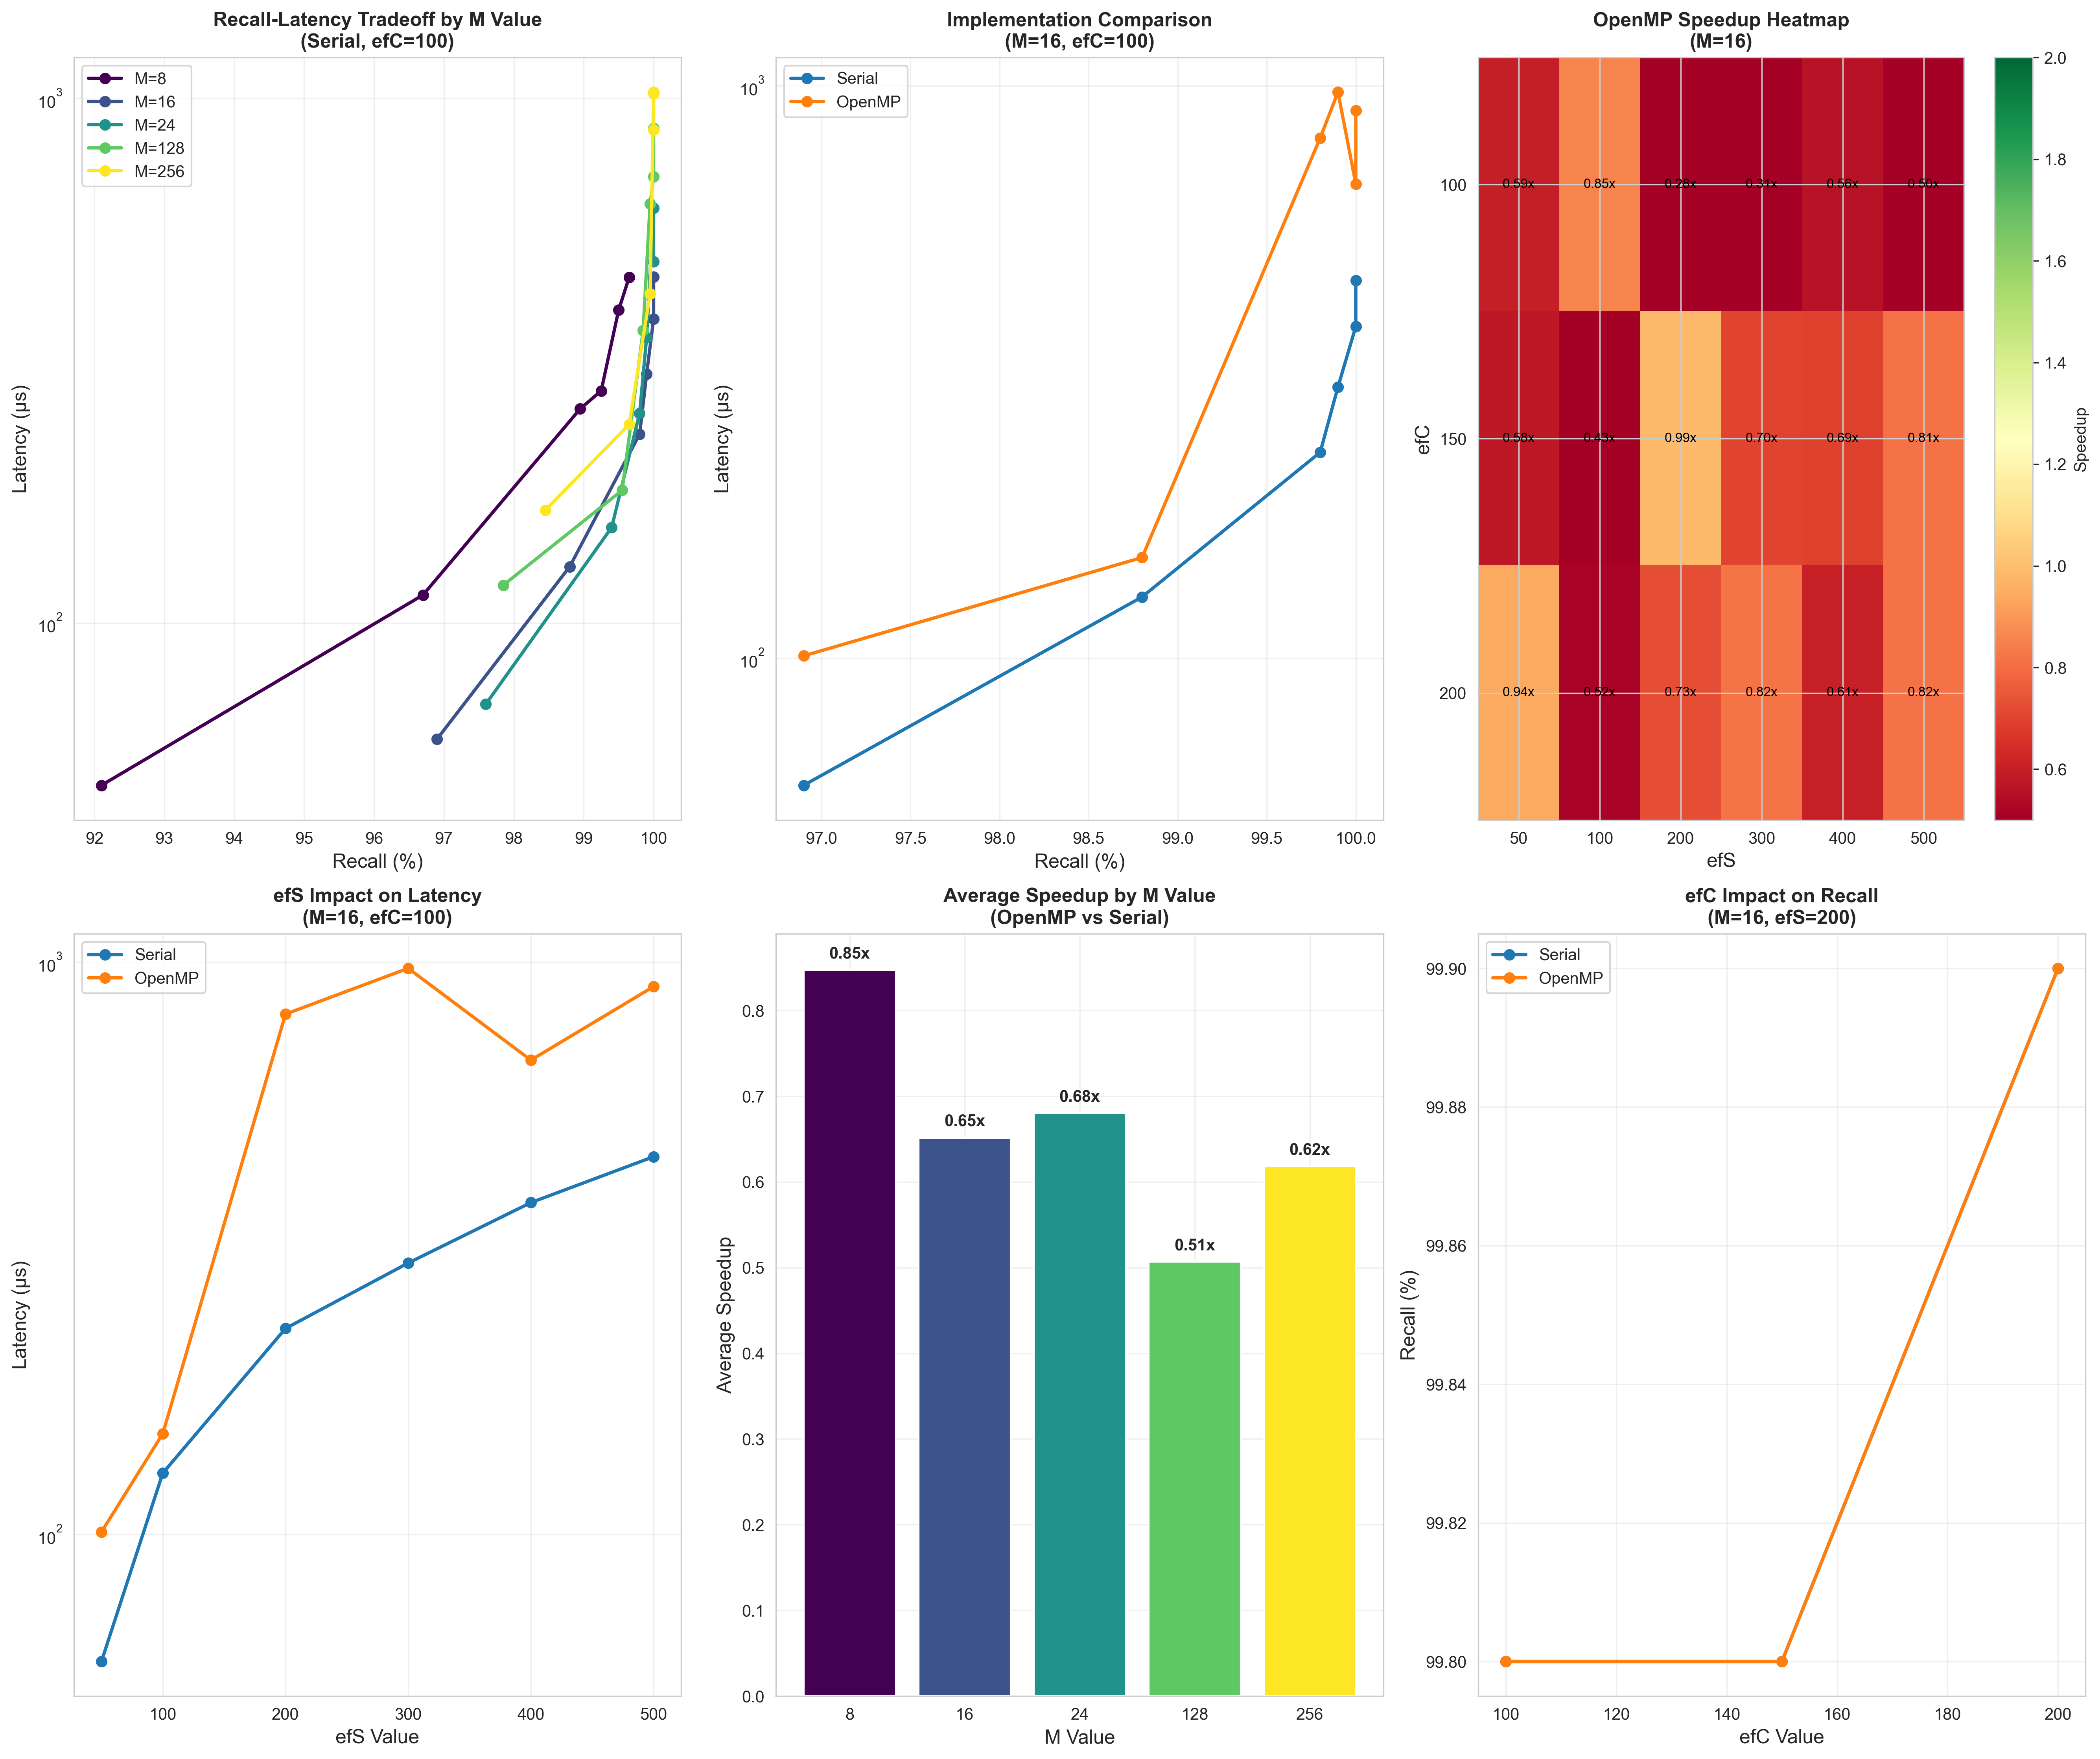
\includegraphics[width=\textwidth]{plots/hnsw_comprehensive_analysis_en.png}
\caption{HNSW Algorithm Multi-threading Implementation Comprehensive Analysis}
\label{fig:hnsw_comprehensive_en}
\end{figure}

Key observations from the analysis:
\begin{enumerate}
    \item \textbf{M Value Impact}: Smaller M values (8, 16) provide better latency performance, while larger M values (128, 256) help improve recall rates
    \item \textbf{Implementation Comparison}: In most configurations, OpenMP version shows higher latency than the serial version
    \item \textbf{Speedup Heatmap}: Only specific parameter combinations (such as certain M=8 configurations) achieve limited speedup effects with OpenMP
\end{enumerate}

Figure~\ref{fig:hnsw_parameter_sensitivity_en} further analyzes parameter sensitivity.

\begin{figure}[htbp]
\centering
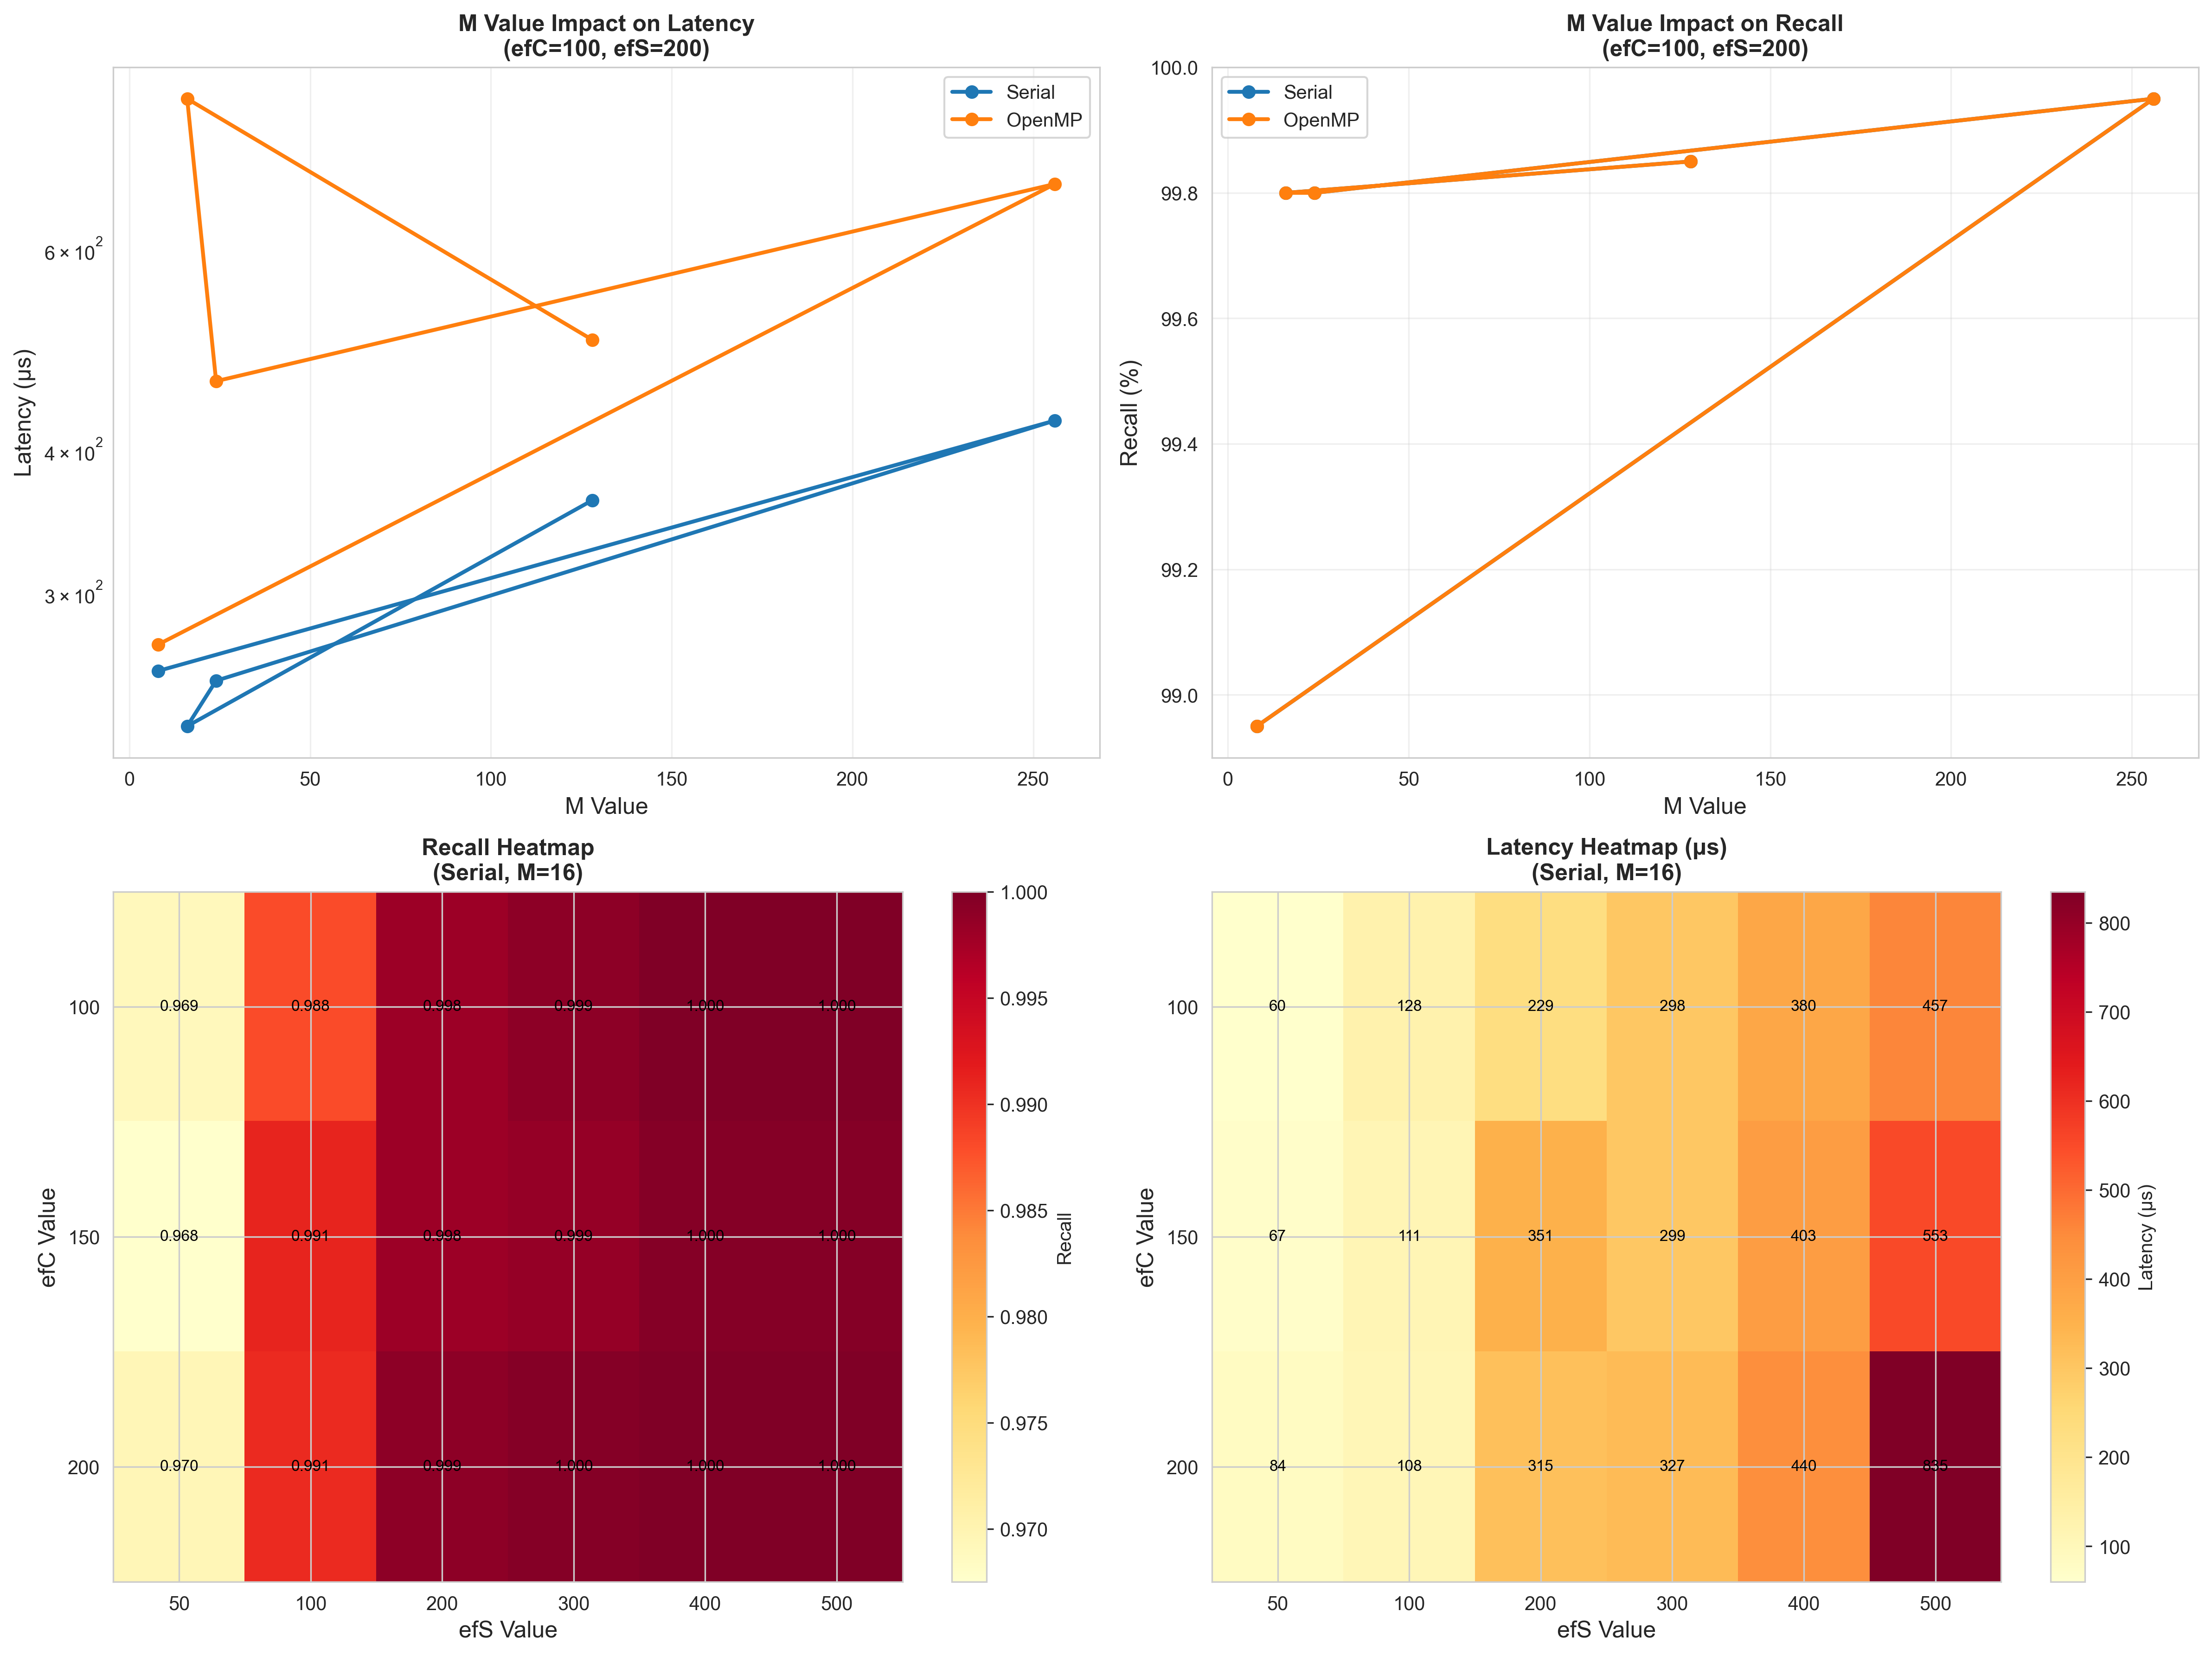
\includegraphics[width=\textwidth]{plots/hnsw_parameter_sensitivity_en.png}
\caption{HNSW Algorithm Parameter Sensitivity Analysis}
\label{fig:hnsw_parameter_sensitivity_en}
\end{figure}

\paragraph{Optimal Configuration Recommendations}

Based on experimental results, we recommend the following configurations for different application scenarios:

\textbf{High Recall Scenarios (Recall ≥ 99.9\%):}
\begin{enumerate}
    \item Serial: M=16, efC=100, efS=300 (Recall=99.90\%, Latency=298μs)
    \item Serial: M=16, efC=200, efS=200 (Recall=99.90\%, Latency=315μs)
    \item Serial: M=16, efC=200, efS=300 (Recall=99.95\%, Latency=327μs)
\end{enumerate}

\textbf{Low Latency Scenarios (Recall ≥ 95\%):}
\begin{enumerate}
    \item Serial: M=16, efC=100, efS=50 (Recall=96.90\%, Latency=60μs)
    \item Serial: M=16, efC=150, efS=50 (Recall=96.75\%, Latency=67μs)
    \item Serial: M=24, efC=100, efS=50 (Recall=97.60\%, Latency=70μs)
\end{enumerate}

\subsubsection{Multi-threading Implementation Challenges}

The poor performance of HNSW algorithm's OpenMP parallelization stems from several key factors:

\begin{enumerate}
    \item \textbf{Algorithm Characteristics}: HNSW search is an iterative graph traversal process where each step's search direction depends on previous results, creating strong data dependencies that resist effective parallelization.
    
    \item \textbf{Memory Access Patterns}: The irregular memory access patterns of graph structures lead to low cache hit rates, with significant cache coherence overhead in multi-threaded access scenarios.
    
    \item \textbf{Thread Synchronization Overhead}: Ensuring search result correctness requires thread synchronization at critical paths, introducing additional overhead.
    
    \item \textbf{Load Imbalance}: Varying search complexity across different layers leads to uneven load distribution among threads.
\end{enumerate}

\subsubsection{Multi-threading Optimization Summary}

Based on experimental results, we conclude:

\begin{enumerate}
    \item \textbf{HNSW Algorithm Unsuitable for Simple OpenMP Parallelization}: Due to inherent algorithm characteristics, OpenMP parallelization not only fails to improve performance but causes significant performance degradation.
    
    \item \textbf{Serial Version Recommended}: Under current implementation conditions, the serial version provides optimal performance and should be prioritized in practical applications.
    
    \item \textbf{Parameter Tuning Importance}: Proper parameter configuration (especially M and efS values) achieves good balance between recall rate and latency.
    
    \item \textbf{Advanced Parallelization Strategies Needed}: Effective HNSW parallelization requires more sophisticated parallel strategies, such as batch query parallelism, data parallelism, or pipeline parallelism.
\end{enumerate} 